\chapter{The way to get better results}
In this chapter described several approaches to improve genetic solver to solve more complex problems.
To do this, a benchmark measurement was made.
We concentrate on solving the problem with parameters:
\begin{itemize}
	\item variants: 10,
	\item depth: 2,
	\item requests: 15,
	\item resources: 5,
	\item timeout: 5 minutes.
\end{itemize}.
Due to the problem, the basic version of the genetic solver could not solve this problem at all. We do all this work to, firstly, achieve valid results, and then get a near-optimal solution. 
All measurements here and later were done at least five times. 
Figure~\ref{label} shown the box-plot of number of contract violation in basic version~\footnote{As a basic version taked version from 24.09.2019, commit: 57845c126c30a1ea59cb35eb16af0bd37930dda9} of genetic solver, as shown there are no valid results cause no results with zero contract violations.

\begin{figure}
	\centering
	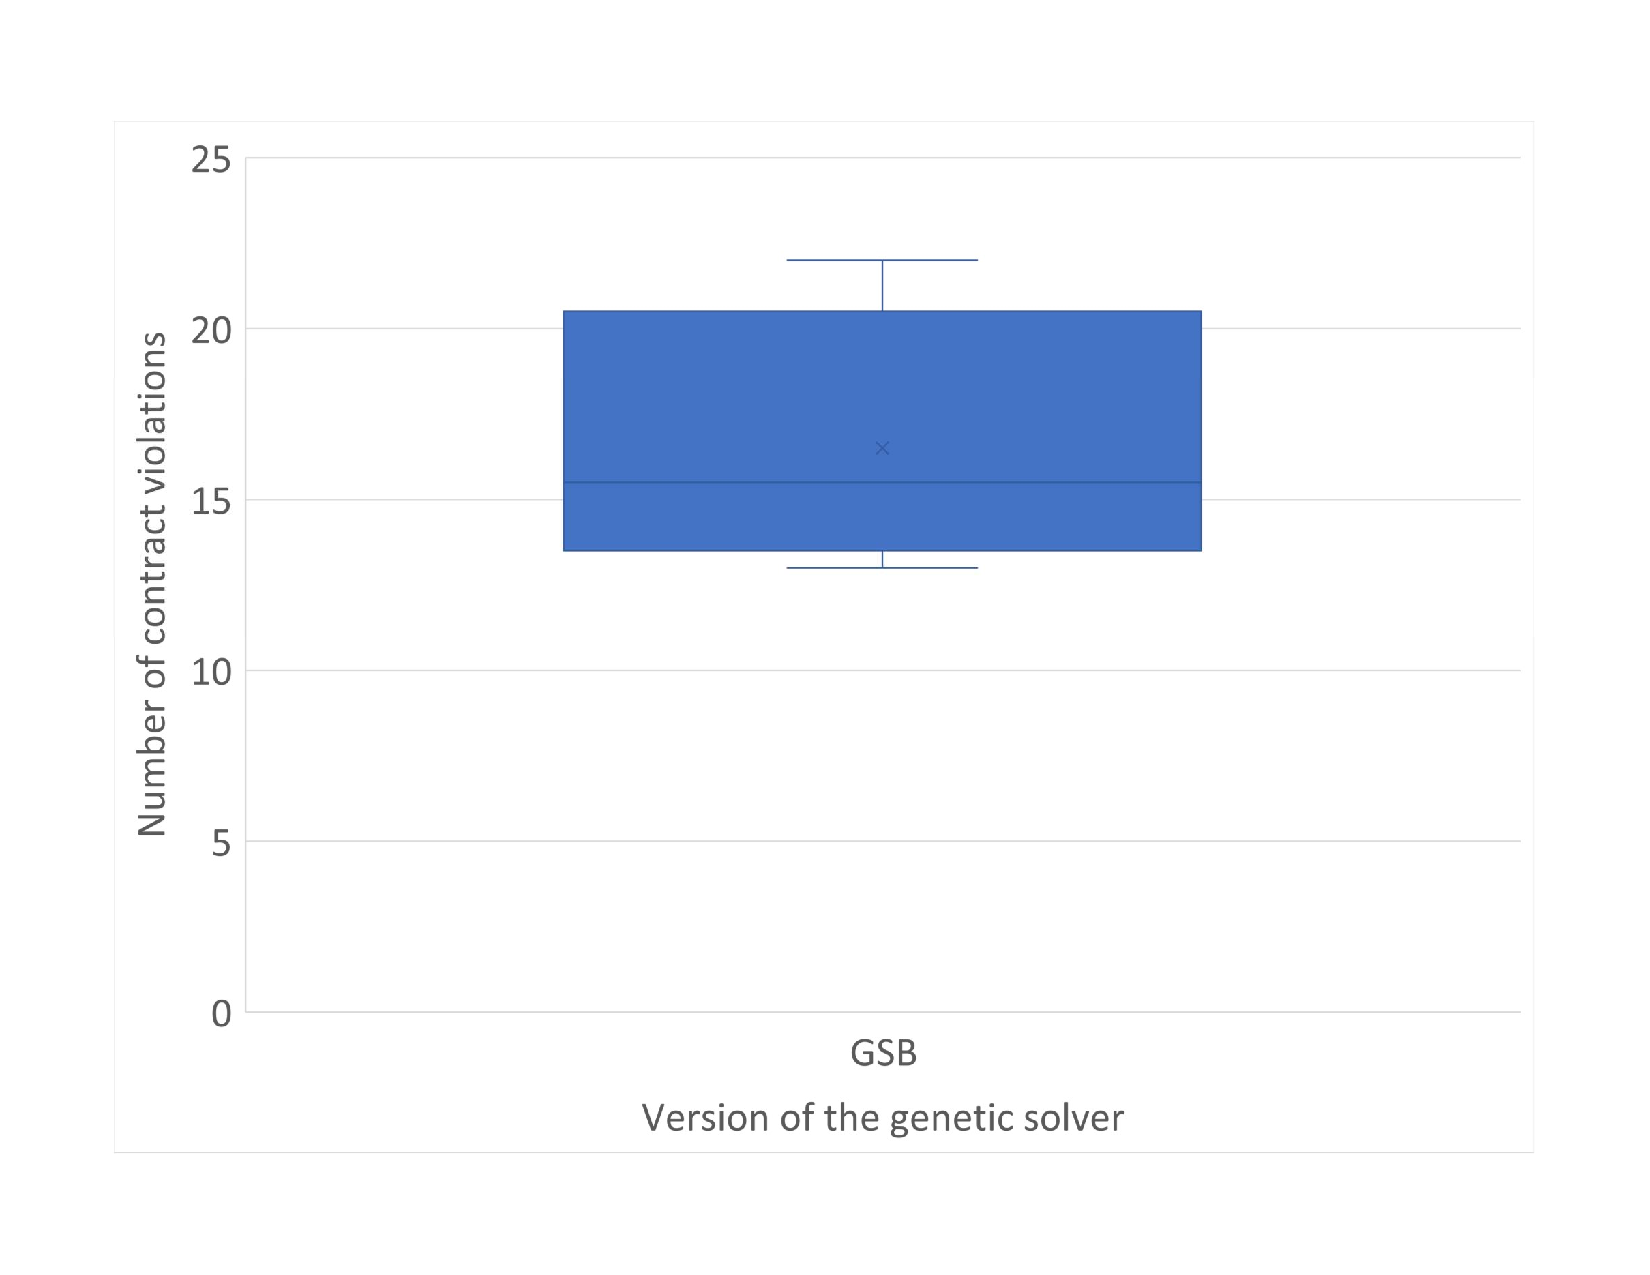
\includegraphics[width=\textwidth]{images/BoxPlotSolverBasic}
	\caption[Boxplot with a number of contract violations for the basic version of genetic solver]{}
	\label{fig:boxplotsolverbasic}
\end{figure}


\section{Parameter tuning as a beginning of live}\todo{new title}
The first step to improve the genetic solver was a parameter optimization. To perform parameter optimization was performed a few important steps.
\begin{enumerate}
	\item Analysis of genetic solver to find out all parameters that could be changed. 
	\item Adapt BRISE to work with the genetic solver.
	\item Prepare Experiment description for BRISE.
	\item Run BRISE to get the optimal configuration.
\end{enumerate}

After deep-diving into the code of genetic solver, the list of parameters was prepared.
In the basic version of the genetic solver, there are only three parameters that are changeable on call. There are:
\begin{itemize}
	\item selectorType - type of the selector algorithm that was mentioned in section~\ref{sec:GeneticAlgorithm:Selector},
	\item number of generation - number of generations that performed by the genetic solver, working as a termination condition, in this thesis we use only timeout termination, so this parameter set as a huge value,
	\item PopulationSize - number of individuals in a population.
\end{itemize}

Adaptation of genetic solver to work into a BRISE consist of a few steps:
\begin{enumerate}
	\item prepare executable file of genetic solver,
	\item implement a method for a worker that will call the file from the previous step and returns the results with a number of contract violations and energy consumption.
\end{enumerate}

Step number 3 means that the user describes parameters that need to optimize, their names, ranges if the parameter has continuous range, or all variants if categorical. The user also should set what components to use, what the minimal number of measurements of a single Configuration, etc.
For parameter optimization of genetic solver, we use the experiment description shown in \todo{appendix or here?}.

When optimal configuration was founded, we use it to analyze results in a boxplot.
The results showed on Figure~\ref{fig:boxplotsolverbasictuning}.
\begin{figure}
	\centering
	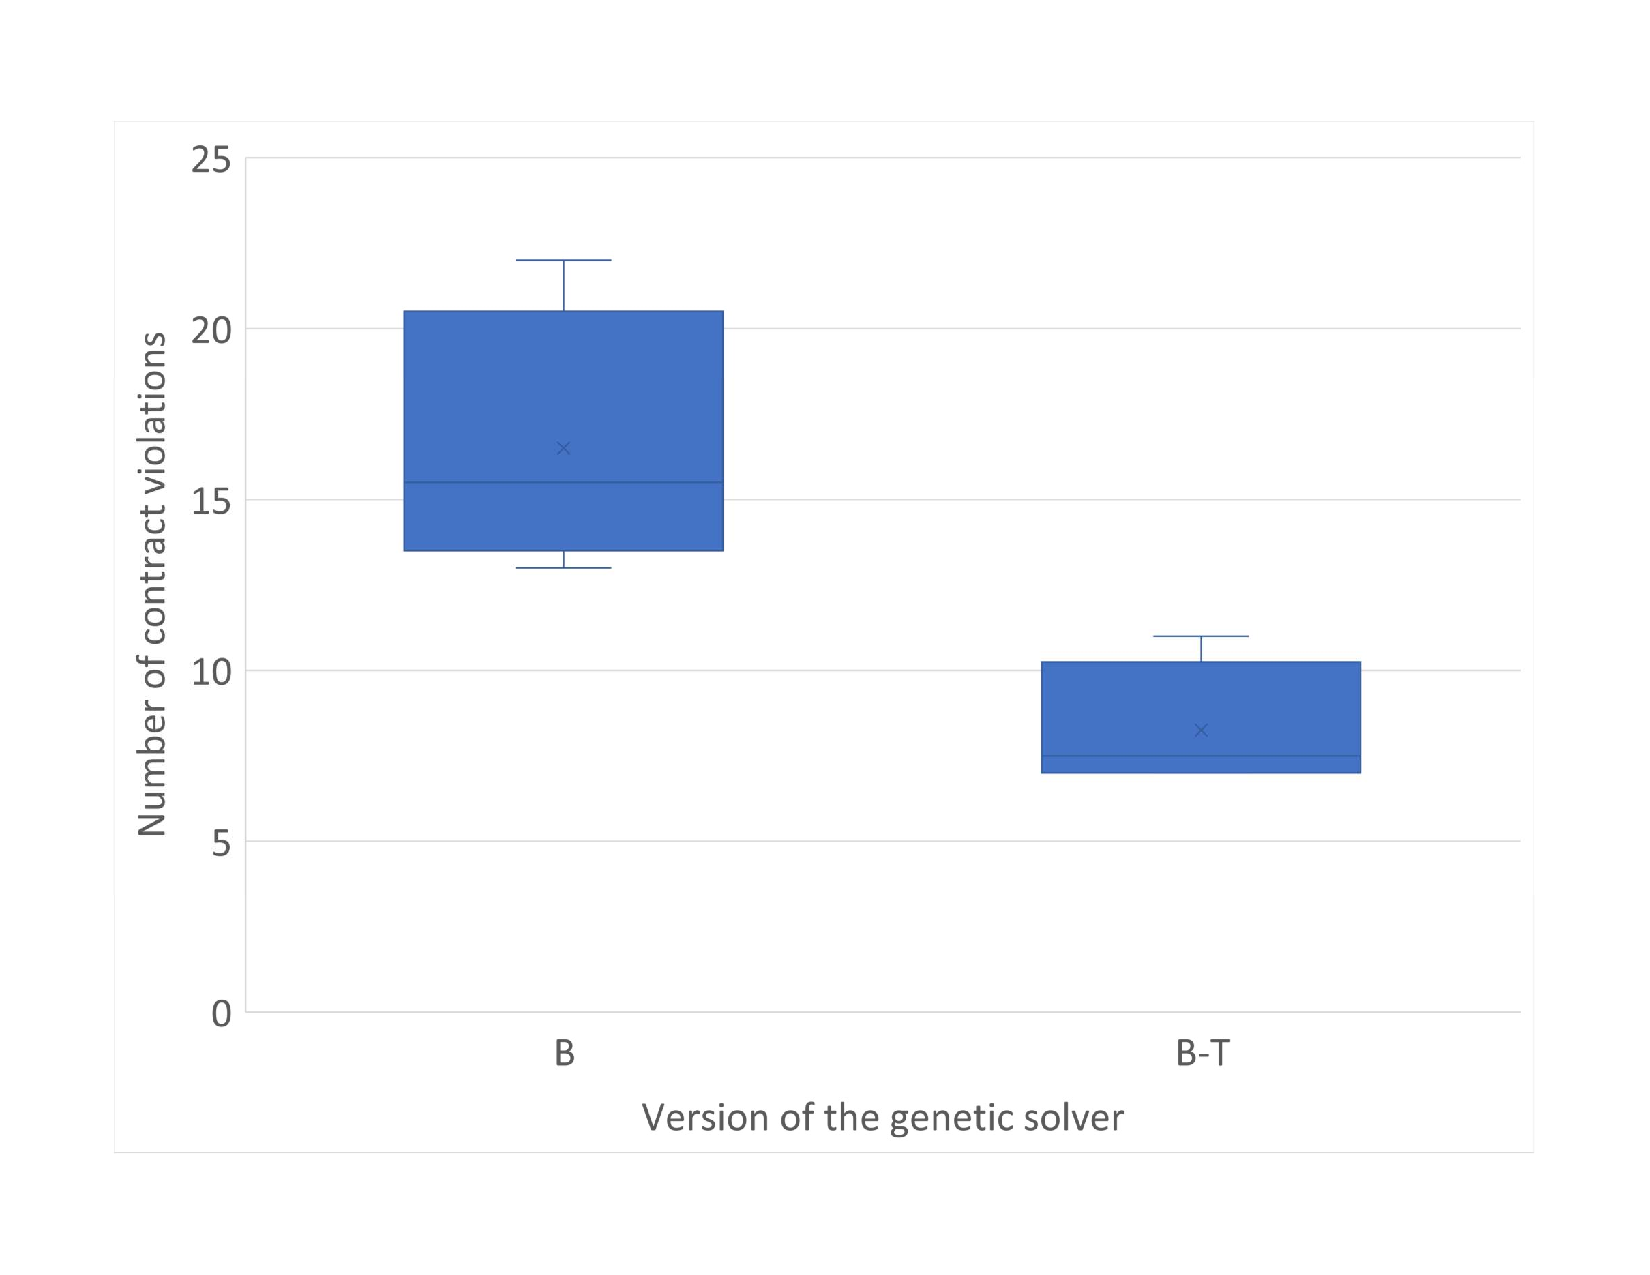
\includegraphics[width=\textwidth]{images/BoxPlotSolverBasicTuning}
	\caption[Boxplot with a number of contract violations for the basic version of genetic solver and with tuned parameters]{}
	\label{fig:boxplotsolverbasictuning}
\end{figure}

Conclusions of this step:
\begin{enumerate}
	\item All results still not valid.
	\item Number of contract violations is less.
	\item The distance between max and min result is smaller.
\end{enumerate}

\section{What if we could change magic numbers or Explain the code to ducks}
Previous section show that even with good set of parameters genetic solver could not get valid results.
After more detailed analysis of code we found out more parameters, that has static values:
\todo{Should I put here a screenshot from the code?}
\begin{itemize}
	\item lambda - the number of new the number of new offspring individuals per generation,
	\item CrossoverRate - as mentioned in section~\ref{sec:GeneticAlgorithmCrossover}, it describes the probability of two individuals to exchange their genes,
	\item mu - the number of parents, that selected by selector to create new individuals,
	\item MutationRate - as mentioned in section~\ref{sec:GeneticAlgorithmMutation}, it describes the probability of the individual to mutate,
	\item Resource Mutation Probability - the probability that during mutation mapped resource will mutate,
	\item CrossoverProbability - probability to do crossover inside crossover operator,\todo{so stupid}
	\item ValidityWeight - coefficient that shows how each contract violation degrees the quality of the solution, 
	\item SoftwareValidityWeight - coefficient that shows how each error in software tree degrees the quality of the solution,
	\item RandomSoftwareAssignmentAttempts - max number of attempts to set a valid software tree to individual on creation phase,
	\item populateSoftwareSolutionAttempts -  max number of attempts to assign software component and resource to get a valid individual on creation phase.
\end{itemize}

To made them changeable we use \textit{GoogleGuiceDependencyInjection} to change values of this parameters during the solver call.

Figure~\ref{fig:boxplotsolverNoHardcodedTuning} shows the results of genetic solver with all parameters after optimization in BRISE.
\begin{figure}
	\centering
	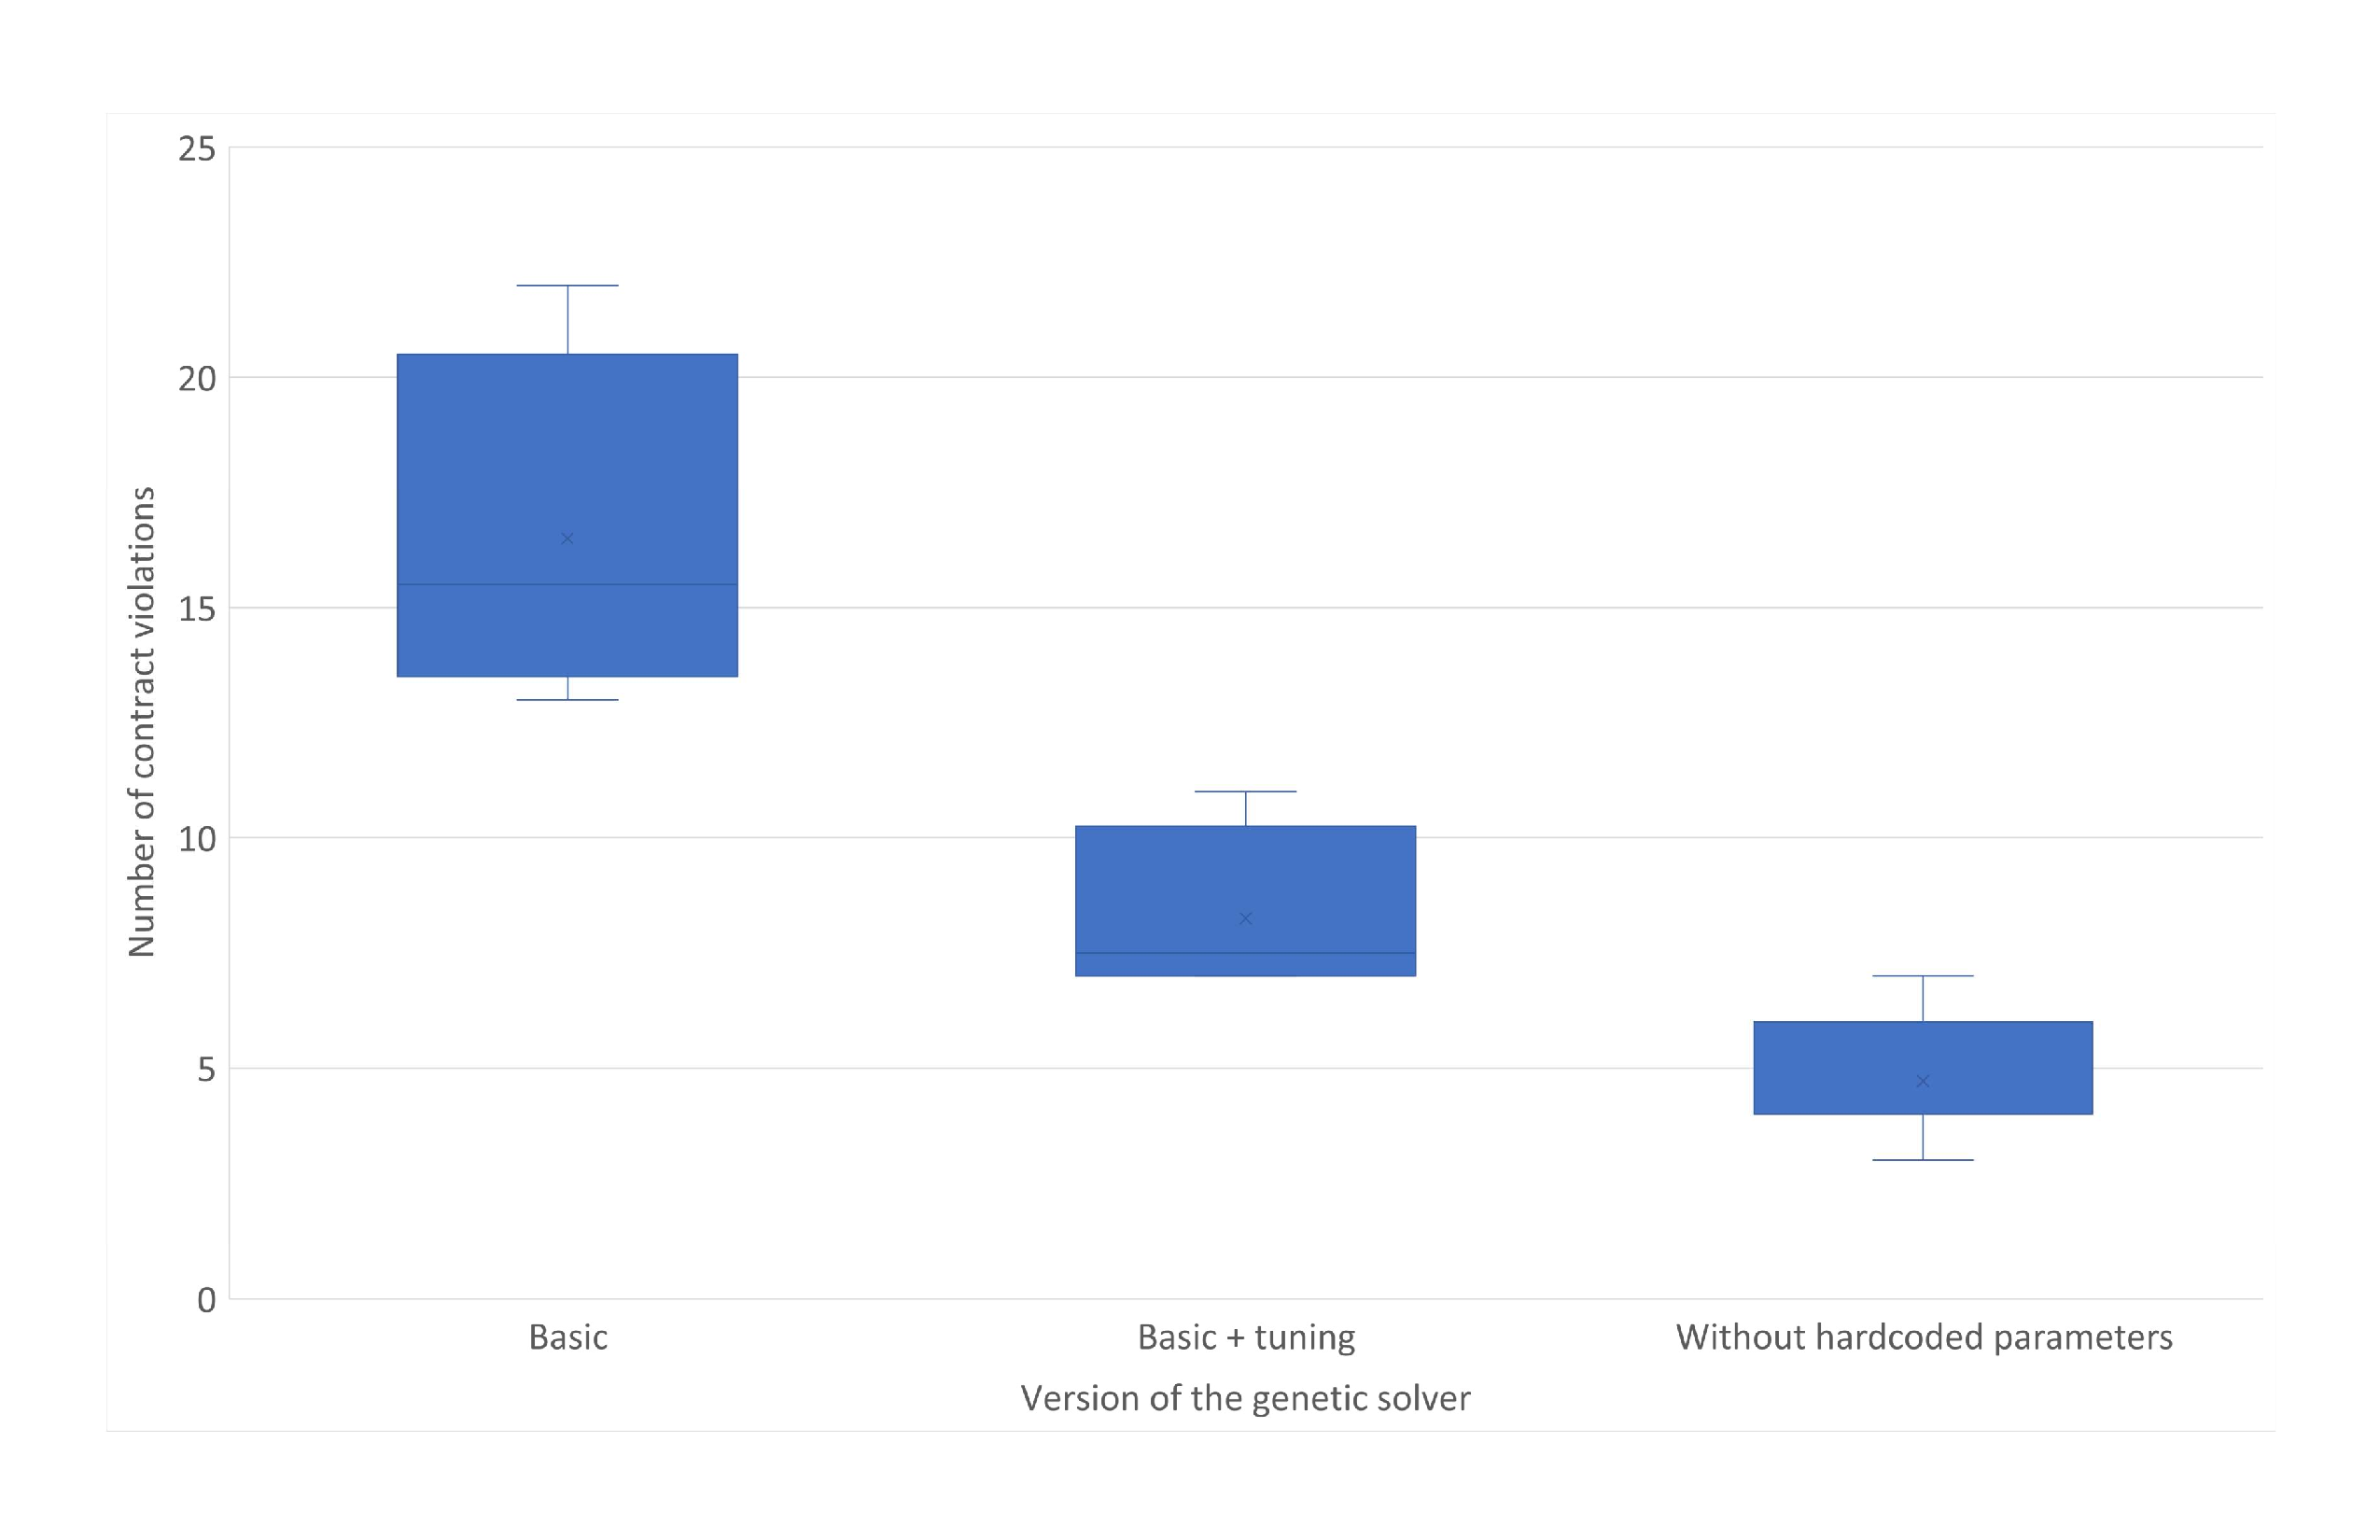
\includegraphics[width=\textwidth]{images/BoxPlotSolverNoHardcodedTuning.pdf}
	\caption[Boxplot with a number of contract violations for the genetic solver without hardcoded parameters]{Boxplot with a number of contract violations for the genetic solver without hardcoded parameters}
	\label{fig:boxplotsolverNoHardcodedTuning}
\end{figure}
Results a bit better but still without valid results.
This step confirms the fact that good values of parameters have a big influence on the results, but sometimes parameter tuning not enough to get good results.
That's the time when we need good parameter engineering. 

\section{Astrologers have announced a week of probabilities. The number of probabilities doubled.}
if you look more detailed in the implementation of the crossover and mutation you will find out that crossover point and mutation point are pretty static.
In crossover:
\begin{itemize}
	\item after the check it recursively goes down and swap both children and their sub-trees,
	\item recombination applied on all requests of the genotype,
	\item crossover point depends on checks of the same nodes of trees.
\end{itemize}

To made crossover and mutation points are more random we add more probabilities that moves them in different ways.
There are:
\begin{itemize}
	\item Crossover On Random Child Probability
	\item Crossover On Random Level Probability
	\item Crossover On Random Request Probability
	\item Mutation On Random Child Probability
	\item Mutation On Random Request Probability
\end{itemize}


\section{Peppa Pig and adaptation for own life}
adaptive CrossoverRate and how it works


\section{Unique genotypes is a God sign or placebo for genetic algorithms}
How works unique individuals in a population

\section{Bermuda Triangle and Missing Parameters}
MAYBE there will be information about not important parameters

\section*{Conclusion - Today we dried coals using the oven in Aleksandrovka}
Combination of different techniques and optimizations could give you better results 